\subsection{Heat maps}\label{heatmaps}

\subsubsection{Definition}\label{heatmapdefinition}

A heat map is a two dimensional graphical representation of a matrix using colours to correspond to different magnitudes of values. It is a thematic map of a matrix, although can also be applied to geographical maps. 

\begin{figure}[H]
        \begin{center}
                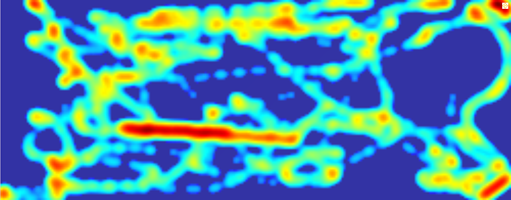
\includegraphics[scale=0.5]{./images/heatmaps/ExampleMouseMove.png}
                \caption{Example heat map generated from mouse movements}
                \label{fig:mousemoveheatmap}
        \end{center}
\end{figure}

Heat maps are generally used to quickly display which values in a matrix have the greatest magnitude and how they compare to surrounding values. Figure~\ref{fig:mousemoveheatmap}, which represents mouse movements on a website clearly shows a horizontal band in the middle which indicates that the users mouse spent a lot of time there. 

\paragraph{Calculations and Colour Progression} \hspace{0pt} \\


In order to create an image representation of the matrix, a colour progression must be chosen. The simplest colour progression method is a hue change on a single colour corresponding to the information. However this may not always be the most suitable method. When giving out information to the public, certain colours tend to represent different things. Red normally has negative connotations while green is the opposite. For this we can use a blended hue colour progression with red at one end of the scale and green at the other.

The algorithm to generate the colour range is very simple. In python for red to green we get the following code (the method accepts a normalised value):


\begin{minted}{python}	
	def value_to_rg(v):
	    oR = 255.0 * (1.0 - v)
	    oG = 255.0 * v
	    return '#%02x%02x%02x' % (oR, oG, 0)
	    
	print value_to_rgb(0.5) #returns '#7f7f7f'
\end{minted}


\paragraph{Representation Matrix} \hspace{0pt} \\

In order to generate the heat map we first need a matrix. A simple matrix can generate an effective heat map as can be seen from the following example.

\begin{figure}[H]
        \begin{center}
                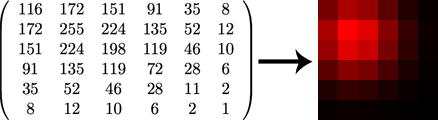
\includegraphics[scale=0.5]{./images/heatmaps/HeatMapGaussianExample.png}
                \caption{Heat Map Generation Example}
                \label{fig:matrixheatmapexample}
        \end{center}
\end{figure}

The example in figure~\ref{fig:matrixheatmapexample} has the maximum value of 255 represented by red (RGB value of \#FF0000) and the minimum value of 1 being almost black (RGB value \#010000). 

\emph{Missing Values}

With many applications there are either missing values in the matrix, or the values cannot be easily placed into a matrix (as is the case for geographical readings). To find the missing values, interpolationof some kind is used. In the above figure the matrix was generated by placing the value 255 in position (2,2) and performing a gaussian blur with a filter size of 2 by 2 pixels and sigma equal to 2. 

Irregular data points must be processed further by mapping them onto a matrix. In the case of taking geographical readings, the heat map can be regenerated for each zoom level to ensure the maximum accuracy. 

These methods are not completely accurate and the missing data should be calculated in a manner appropriate to the application.

\subsubsection{Applications in Air Quality Measurement}\label{applicationsinaqmeasurement}

Heat maps are extremely useful to show the concentrations of pollutants in geographical areas. The information is easily given when overlaid on top of a map.  

\begin{figure}[H]
        \begin{center}
                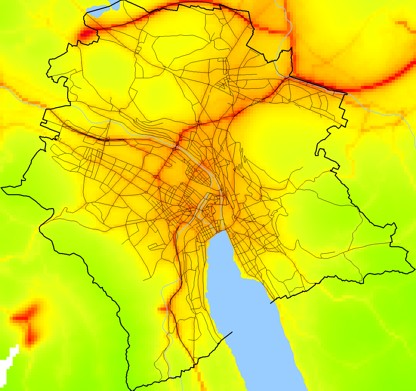
\includegraphics[scale=0.5]{./images/heatmaps/zurichpm.jpg}
                \caption{Particulate matter heat map in Zurich. Source: \url{www.stadt-zuerich.ch}}
                \label{fig:pmheatmapzurich}
        \end{center}
\end{figure}

From the above image we an easily see that the highest concentrations of particulate matter are where the roads are situated indicating a relationship between the two. 




